% !TeX encoding = UTF-8
% !TeX root = choix_extensions.tex
\chapter{Prise en main}






\section{Introduction}

Ce document décrit comment mettre en place un environnement de travail \LaTeX \ fonctionnel basé sur la distribution \TeX \ Live, l'éditeur TeXstudio et les fichiers de style \incmd{preambule_college.sty} et \newline
\incmd{preambule_personnalisation.sty}. Il regroupe des trucs et astuces qui m'ont pris du temps à trouver et à mettre au point. En cas de remarque : \href{mailto:samuel.vannay@edu.vs.ch}{samuel.vannay@edu.vs.ch}.



\subsection{Pour les impatients}


\subsubsection{Pour commencer sans distribution}

Pas besoin d'installer quoi que ce soit pour commencer à apprendre les bases de \LaTeX. Il suffit d'essayer en ligne sur
\begin{center}
	\href{https://www.learnlatex.org/fr/}{Learn\LaTeX.org}.
\end{center}

Pas besoin non plus d'installer quoi que ce soit pour commencer à travailler. Il suffit de créer un compte sur
\begin{center}
	\href{https://www.overleaf.com/}{Overleaf}.
\end{center}


\subsubsection{Installer et configurer}

Installations requises :
\begin{enumerate}
	\item \TeX \ Live avec toutes ses collections (cf. captures dans la fiche \emph{Mise en place de son environnement de travail});
	\item TeXstudio;
	\item optionnellement, pour ceux qui doivent mettre en forme du code informatique, Anaconda pour avoir Python avec la librairie Pygments.
\end{enumerate}

Configurations à faire à la main :
\begin{enumerate}
	\item Dans TeXstudio (cf. captures \ref{sec:installationTl}) :
		\begin{itemize}
			\item au besoin rajouter les options de compilation \incmd{-shell-escape} et \incmd{-8bit} aux compilateurs;
			\item choisir \XeLaTeX \ comme compilateur par défaut;
			\item choisir \incmd{biber} comme outil de bibliographie par défaut.
		\end{itemize}
	\item Copier les fichiers du répertoire \incmd{cwl} dans :
		\begin{itemize}
			\item $\sim$\incmd{/.config/texstudio/completion/user} sous Linux et Mac OS;
			\item généralement dans \lstinline!%APPDATA%\texstudio\completion\user! sous Windows.
		\end{itemize}
\end{enumerate}


\subsubsection{Utilisation}

Dans TeXstudio :

\begin{enumerate}[a.]
	\item Placer le répertoire \incmd{styles} au même endroit que le document principal.
	\item Personnaliser \incmd{style/preambule_personalisation.sty}, notamment les mots-clés pdf.
	\item Dans le document principal appeler \inlatex{\usepackage[informatique]{styles/preambule_college}} avec ou sans l'option informatique, et \inlatex{\usepackage{styles/preambule_personnalisation}}
		\attention L'option \incmd{informatique} nécessite qu'une distribution Python avec la librairie Pygments soit installée.
	\item Utiliser les exemples de ce document pour les mises en page particulières.
	\item Compiler avec \XeLaTeX \ de la dernière version de \TeX \ Live.
\end{enumerate}





\newpage






\section{Distribution \LaTeX}
\label{sec:distributionLaTeX}







\subsection{Choix de la distribution}

La distribution la plus portable et qui contient uniquement des extensions libres est
\begin{center}
	\href{http://www.tug.org/texlive/}{\TeX \ Live}.
\end{center}

Pour plus de détails, consultez la \href{http://tug.org/texlive/doc/texlive-fr/texlive-fr.pdf}{documentation} officielle\footnote{Pour des variantes, voir cet \href{http://tex.stackexchange.com/questions/239199/latex-distributions-what-are-their-main-differences}{article}.}.



\subsection{Lancer l'installation}

\begin{description}
	\item[\textcolor{red}{pour Linux}] ~\\
		Soit une version est déjà présente, soit elle est disponible dans les dépôts. Mais il vaut la peine d'envisager de désinstaller la version présente et d'installer la version originale à la place. \\
		\textbf{Prérequis : } \incmd{perl-tk} et \incmd{whish} \quad (si nécessaire : \incmd{sudo apt install perl-tk whish} ou équivalent).
		\begin{itemize}
			\item En ligne
				\begin{itemize}
					\item Télécharger et décompresser \href{http://mirror.ctan.org/systems/texlive/tlnet/install-tl-unx.tar.gz}{install-tl-unx.tar.gz}.
					\item Exécuter \incmd{sudo ./install-tl gui} dans le répertoire décompressé.
				\end{itemize}
			\item Hors ligne
				\begin{itemize}
					\item Télécharger le \href{http://mirror.ctan.org/systems/texlive/Images/}{fichier ISO};
					\item Copie ce fichier sur l'ordinateur hors ligne;
					\item l'ouvrir et exécuter \incmd{sudo ./install-tl gui} dans le répertoire de base.
				\end{itemize}
		\end{itemize}
	\item[\textcolor{red}{pour Mac}] ~\\
		Télécharger et installer \href{http://www.tug.org/mactex}{MacTeX}.
	\item[\textcolor{red}{pour Windows}] ~\\
		\attention Sous Windows, l'installation peut être bien longue\dots
		\begin{itemize}
			\item En ligne \\
				Télécharger et exécuter \href{http://mirror.ctan.org/systems/texlive/tlnet/install-tl-windows.exe}{install-tl-windows.exe}.
			\item Hors ligne
				\begin{itemize}
					\item Télécharger le \href{http://mirror.ctan.org/systems/texlive/Images/}{fichier ISO};
					\item Transférer ce fichier sur l'ordinateur hors ligne
					\item L'ouvrir\footnote{Sous certaines versions de Windows, il faut éventuellement installer un utilitaire pour lire le fichier .iso, par exemple \href{http://wincdemu.sysprogs.org/}{winCDEmu}.}, clic droit sur \incmd{install-tl-advanced.exe} qui s'y trouve et \newline \incmd{Exécuter en tant qu'administrateur}.
				\end{itemize}
		\end{itemize}
\end{description}



\subsection{Options d'installation}

Une fois le menu d'installation affiché (pareille pour toutes les plates-formes), on choisit ce qu'on veut. Ici : tout sauf les langues dont on ne va pas se servir (voir les captures d'écran \ref{sec:installationTl}).



\subsection{Utilisation de \TeX \ Live}

Facile : on n'y touche pas !

\remarque*{
	Au besoin, on peut ajouter et retirer des packages avec l'utilitaire \incmd{tlmgr} (voir \ref{sec:majTl}) fourni avec la distribution. Sous Mac OS, cet utilitaire s'appelle \incmd{Tex Live Utility}. \\
	On peut aussi installer la nouvelle version de TeX Live qui sort chaque année au printemps%\dots
}





\section{Éditeur}
\label{sec:Editeur}



\subsection{Choix de l'éditeur}

Le meilleur éditeur libre, offrant exactement la même interface pour Linux, Mac OS et Windows, complet et personnalisable est 
\begin{center}
	\href{http://www.texstudio.org/}{TeXstudio}.
\end{center}

Sa prise en main est rapide\footnote{Pour des alternatives, consultez cet \href{https://en.wikipedia.org/wiki/Comparison_of_TeX_editors}{article} Wikipédia.}.



\subsection{Installation}

\href{http://www.texstudio.org/}{Télécharger} la dernière version et exécuter l'installateur \emph{après} avoir installé \TeX \ Live. De cette manière, il s'intègre à \TeX \ Live tout seul comme un grand.



\subsection{Configuration}

Dès que TeXstudio est installé, il faut faire quelques configurations dans le menu
\begin{center}
	\incmd{Options} \textrightarrow \ \incmd{Configurer TeXstudio...} \quad (ou équivalent sous Mac OS)
\end{center}
Voir les captures de \ref{sec:configTeXstudio}.


\subsubsection{Activer l'appel des scripts externes}

Pour autoriser TeXstudio à appeler des scripts externes comme Pygments, il faut ajouter une option dans la commande qui est passée au compilateur dans la boîte de dialogue \incmd{Configurer TeXstudio}, partie \incmd{Compilations}, rajouter dans les lignes \incmd{PDFLaTeX}, \incmd{XeLaTeX} et \incmd{LuaLaTeX} l'option
\begin{center}
	\incmd{ -shell-escape } \quad (espace avant et espace après)
\end{center}


\subsubsection{Accepter les caractères sur 8 bits}

Pour permettre à \TeX \ Live de gérer sans souci les caractères sur 8 bits, rajouter l'option à vos compilateurs.
\begin{center}
	\incmd{ -8bit } \quad (espace avant et espace après, pas de "s")
\end{center} 


\subsubsection{Choix du compilateur par défaut}

Le compilateur est le logiciel fourni dans \TeX \ Live qui transforme le code \LaTeX \ en document pdf. Il en existe plusieurs : \LaTeX, PDF\LaTeX, Lua\LaTeX \dots

Ici le choix est d'utiliser
\begin{center}
	\XeLaTeX \quad (prononcer Zee Lay Tech).
\end{center}

Ce compilateur prend en charge les caractères Unicode (notamment l'encodage UTF-8 qui est devenu le standard sur tous les ordinateurs) et permet d'utiliser les polices de caractères vectorielles de son ordinateur.

\begin{center}
	\incmd{Configurer TeXstudio} \textrightarrow \ \incmd{Production} \textrightarrow \  \incmd{XeLaTeX} comme compilateur par défaut (voir \ref{sec:configTeXstudio}).
\end{center}


\subsubsection{Réglage de l'auto-complétion}
	
Le fichier \incmd{preambule_college.sty} contient de nombreuses nouvelles commandes. Il est possible de les déclarer à TeXstudio de manière à ce qu'elles apparaissent dans l'auto-complétion et l'analyseur syntaxique. Pour cela, il faut créer un fichier \incmd{cwl} (voir le fichier \incmd{preambule_college.cwl} fourni) et le placer dans le répertoire :
\begin{itemize}
	\item $\sim$\incmd{/.config/texstudio/completion/user} sous Linux et Mac OS;
	\item généralement dans \lstinline!%APPDATA%\texstudio\completion\user! sous Windows.
\end{itemize}

Ensuite, TeXstudio peut charger ce fichier \incmd{.cwl} automatiquement, mais pour s'assurer que c'est chaque fois le cas, il vaut mieux l'activer manuellement dans :
\begin{center}
	Menu \incmd{Options} \textrightarrow \ \incmd{Configurer TeXstudio} \textrightarrow \ Onglet \incmd{Complétion}
\end{center}



%\subsubsection{Mise en place du modèle de polycopié}
%
%Il est possible de faire des modèles de document et de les déclarer à TeXstudio. Un modèle de polycopié a été préparé pour faciliter la création de document multi-fichiers. Pour l'activer, il faut copier les fichiers \newline \incmd{template_polycop.zip}, \incmd{template_polycop.json} et \incmd{template_polycop.png} dans le répertoire :
%\begin{itemize}
%	\item $\sim$\incmd{/.config/texstudio/template/user} sous Linux et Mac OS;
%	\item généralement dans \lstinline!%APPDATA%\texstudio\template\user! sous Windows.
%\end{itemize}






\section{Produire un code maintenable}

Avec \LaTeX \ on sépare le contenu de la forme. Le principe de base en \LaTeX \ est donc le suivant :

\begin{center}
	\begin{boxedminipage}{.75\textwidth}
		\textcolor{red}{\textbf{Utilisez \emph{systématiquement} des raccourcis (les créer au besoin) qui décrivent le contenu et non la mise en forme.}}
		
		\textcolor{red}{Le fichier \incmd{preambule_college.sty} contient une quantité de raccourcis de ce type qu'il faut utiliser systématiquement. Ce document les présente en détail.}
	\end{boxedminipage}
\end{center}

Cela permet de modifier ensuite globalement l'apparence d'un document sans avoir à en modifier le contenu. 

\exemple*{	
	Dans les définitions mathématiques, on veut réserver une mise en forme spéciale pour les mots faisant l'objet de la définition. Certains préfèrent les mettre en italique, d'autres en gras. Dans ce cas, on procède de la manière suivante :
	\begin{enumerate}
		\item Convenir d'une balise commune, ici \mintinline{latex}{\emphdef}.
		\item Définir cette balise dans un fichier \incmd{.sty}. Ici, \incmd{preambule_college.sty} contient : \newline
		\mintinline{latex}{\newcommand{\emphdef}[1]{\emph{\#1}}} \footnote{\mintinline{latex}{\newcommand} débute la création d'une nouvelle commande, \incmd{[1]} spécifie qu'on va donner une série de mots en paramètre de la commande. La suite indique de mettre en italique les mots passés en paramètres.}.
		\item Utiliser systématiquement cette balise pour les définitions dans le fichier \incmd{.tex}.
		\item Pour adapter l'apparence des mots définis à ce qu'on veut, il suffit de changer la description de \mintinline{latex}{\emphdef}, ce qui est d'ailleurs le cas dans le fichier \incmd{preambule_personnalisation.sty} : \newline
		\mintinline{latex}{\renewcommand{\emphdef}[1]{\textbf{#1}}} \newline
		Ceci écrase l'ancienne définition et fait afficher les mots définis en gras.
	\end{enumerate}
}




\section{Où placer ses fichiers .sty}



\subsection{Pour éviter tout problème}

Quand on copie le répertoire exemple, tout est prêt pour travailler sans mauvaise surprise : le sous-répertoire \incmd{style} contient les fichiers \incmd{preambule_college.sty} et \incmd{preambule_personalisation.sty}.

De cette manière, on peut personnaliser son document (hiérarchie de la numérotation, mots-clés pour les méta-informations pdf, licences d'utilisation\dots) et si les fichiers de style viennent à évoluer indépendamment de ce document particulier, on a la garantie de pouvoir toujours le compiler avec l'ancienne version des styles.



\subsection{Pour une configuration centralisée}

Il est possible (et déconseillé) de placer les \incmd{.sty} dans un seul endroit d'où ils seront accessibles pour tous les documents. Il y en a qui ont essayé : ils ont eu des problèmes\dots

Les répertoires centraux sont les suivants :
\begin{itemize}
	\item Linux \incmd{~/texmf/tex/latex/local/}
	\item Mac OS X \incmd{<user name>/Library/texmf/tex/latex/local/}
	\item Windows \Verb!C:\Users\<user name>\texmf\tex\latex\local\!
\end{itemize}

Après avoir placé les fichiers dans ces répertoires, il faut encore signaler leur présence à \LaTeX \ soit avec \TeX Live Manager (\incmd{tlmgr}), soit à la ligne de commande (\incmd{texhash}, voire \incmd{mktexlsr}). Voir la  \href{http://tug.org/texlive/doc/texlive-fr/texlive-fr.pdf}{documentation} de \TeX \ Live pour plus d'informations.





\section{Captures d'écran}
\label{sec:captures}



\subsection{Configurer l'installation de \TeX \ Live}
\label{sec:installationTl}

Ces captures ont été faites durant l'installation d'une version \TeX \ Live 2021 sous Linux. C'est quasiment pareil pour Windows et entièrement différent pour Mac\dots

\begin{figure}[H]
	\centering
	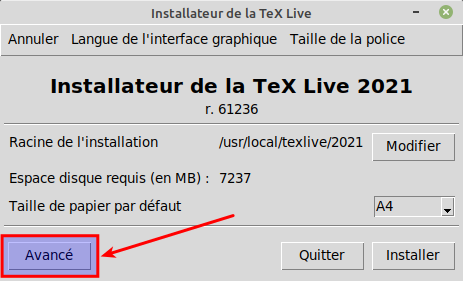
\includegraphics[width=6cm]{captures/install_TL_01.png}
	\caption{Mode avancé}
	\label{fig:captureTLInstall01}
\end{figure}

\begin{figure}[H]
	\centering
	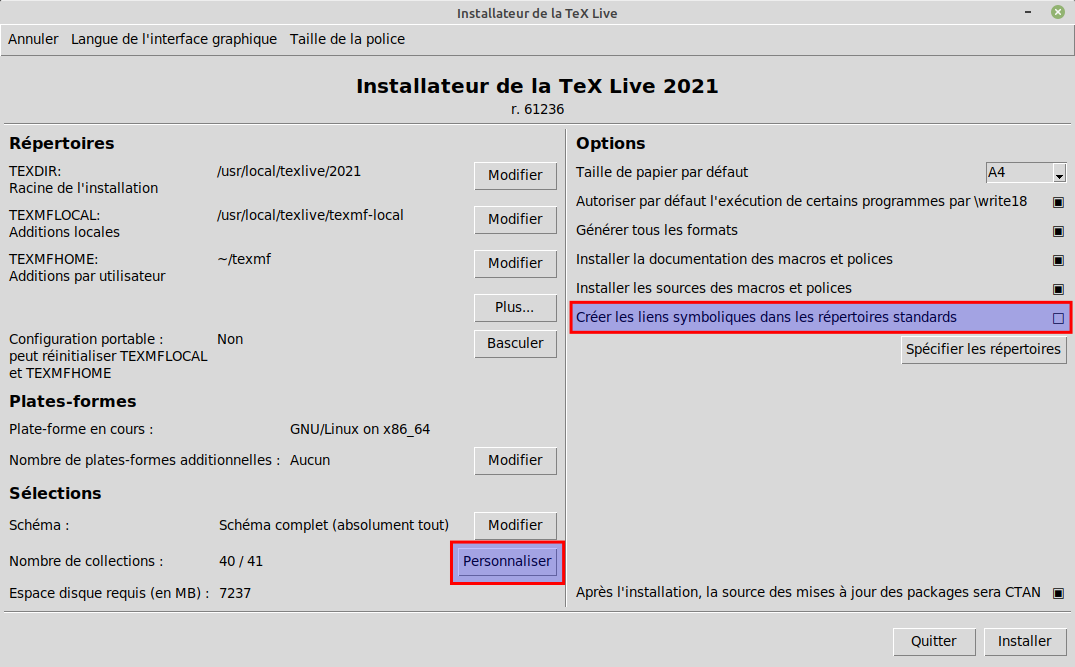
\includegraphics[width=15cm]{captures/install_TL_02.png}
	\caption{Faire créer les liens et choisir les collections}
	\label{fig:captureTLInstall02}
\end{figure}

\begin{figure}[H]
	\centering
	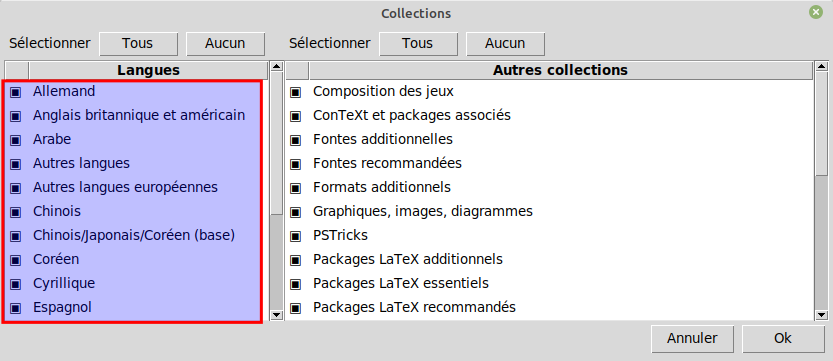
\includegraphics[width=10cm]{captures/install_TL_03.png}
	\caption{Ne garder que le français}
	\label{fig:captureTLInstall03}
\end{figure}



\subsection{Mettre \TeX \ Live à jour}
\label{sec:majTl}


\subsubsection{Linux et Windows}

\begin{figure}[H]
	\centering
	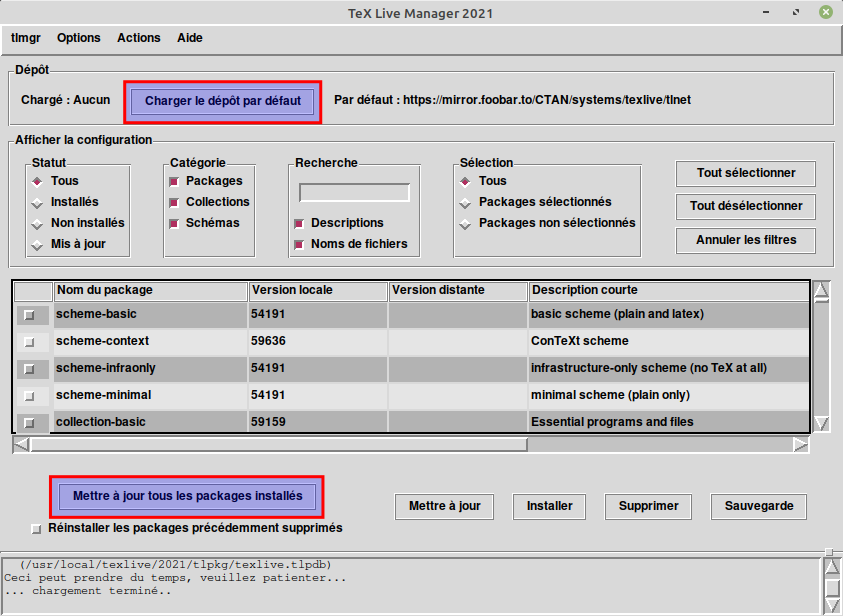
\includegraphics[width=\linewidth]{captures/TL_manager_2021.png}
	\caption{Activer les dépôts et lancer la mise à jour}
	\label{fig:captureTLInstall01}
\end{figure}


\subsection{Configurer TeXstudio}
\label{sec:configTeXstudio}

\begin{figure}[H]
	\centering
	\includegraphics[width=\linewidth]{captures/configurer_TeXstudio_compilations}
	\caption{Configuration de TeXstudio - Compilations}
	\label{fig:captureConfigTeXstudioCompilations}
\end{figure}

\begin{figure}[H]
	\centering
	\includegraphics[width=\linewidth]{captures/configurer_TeXstudio_production}
	\caption{Configuration de TeXstudio - Production}
	\label{fig:captureConfigTeXstudioProduction}
\end{figure}





\subsection{Fichiers fournis}

\begin{enumerate}
	\item \incmd{choix_extensions.pdf} ce document.
	\item \incmd{cwl/} répertoire pour déclarer les raccourcis à TeXstudio.
	\item \incmd{sources/} les sources pour créer ce document.
	\item \incmd{styles/}
	\begin{enumerate}[a.]
		\item \incmd{styles/preambule_college.sty} \\
		choix organisé et commenté d'extensions et de raccourcis utiles pour la mise en forme de documents généraux, mathématiques et informatiques. L'option \inlatex{informatique} permet d'activer les packages et raccourcis pour mettre en page du code informatique. \\
		\attention L'option \inlatex{informatique} requière l'installation de Python et de sa librairie Pygments au préalable. Le plus simple est d'installer \href{https://www.anaconda.com/products/individual}{Anaconda}.
		\item \incmd{styles/preambule_personalisation.sty} \\
		réglages qui sont propres à chaque nouveau document. Ce fichier {\color{red}{\textbf{doit être adapté pour chaque nouveau document.}}}
	\end{enumerate}
\end{enumerate}




